\documentclass[10pt]{article}
\usepackage{tikz}
\usetikzlibrary{shapes.misc}
\usepackage[margin=0cm]{geometry}
\pagestyle{empty}
\tikzstyle{every node}=[cross out, draw, red]

\begin{document}

\vspace*{\fill}
\begin{center}
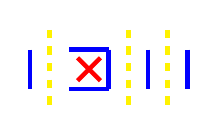
\begin{tikzpicture}[x=0.5cm, y=-0.5cm, ultra thick, blue]
% Walls
    \draw (1,0) -- (2,0);
    \draw (1,1) -- (2,1);
    \draw (0,0) -- (0,1);
    \draw (2,0) -- (2,1);
    \draw (3,0) -- (3,1);
    \draw (4,0) -- (4,1);
% Pillars
% Inner points in accessible cul-de-sacs
    \node at (1.5,0.5) {};
% Entry-exit paths without intersections
    \draw[dashed, yellow] (0.5,-0.5) -- (0.5,1.5);
    \draw[dashed, yellow] (2.5,-0.5) -- (2.5,1.5);
    \draw[dashed, yellow] (3.5,-0.5) -- (3.5,1.5);
\end{tikzpicture}
\end{center}
\vspace*{\fill}

\end{document}
